\chapter{Einleitung}
\label{Einleitung}
Die Skalierung von Software, die auf relationalen Datenbank Management Systemen (RDBMS) basiert, erweist sich in der Praxis als anspruchsvoll. ACID-Eigenschaften (Atomicity, Consistency, Isolation, Durability) dieser Systeme gewährleisten zwar eine hohe Zuverlässigkeit und Datenintegrität, allerdings führen sie auch zu einer Einschränkung der horizontalen Skalierung. \cite{reis2023} Daher erweisen sich diese Systeme bei der Verarbeitung und Analyse von großen Datenmengen (Big Data) in Echtzeit nicht als ausreichend und es sind alternative Lösungsansätze zu evaluieren, um die erhöhten Anforderungen an die Skalierung zu erfüllen.

Die Verarbeitung und Analyse von Big Data ist zwar kein neues Forschungsfeld und es existieren bereits zahlreiche Lösungen und Ansätze in der Literatur. Allerdings ist die Auswahl einer geeigneten Technologie für spezifische Anwendungsfälle keineswegs trivial. Eine sorgfältige Evaluierung ist notwendig, da jede Technologie unterschiedliche Vor- und Nachteile bietet und die Entscheidung von vielen Faktoren abhängt, darunter die spezifischen Anforderungen der Anwendung, die vorhandene Infrastruktur und die gewünschten Performance-Eigenschaften. Die Auswahl der geeigneten Technologien und Architekturen erfordert daher eine gründliche Analyse und Abwägung, um sicherzustellen, dass die Lösung gegenwärtigen und zukünftigen Anforderungen an Flexibilität und Skalierung gerecht wird.

 Die vorliegende Masterarbeit widmet sich dieser Problematik am Beispiel der X4 Business Process Management Software (X4 BPMS), einer Software für die Geschäftsprozessautomatisierung. Ein besonderer Fokus liegt dabei auf den Aspekten der Modularität und Flexibilität bei der Integration in heterogene Systemlandschaften, die sich aus dem Einsatz der Software in unterschiedlichen Branchen und Projekten ergeben. 

\section{Motivation}
Die Motivation dieser Masterarbeit besteht darin, eine flexiblere und skalierbarere Datenmanagementlösung für die X4 Business Process Management Software (X4 BPMS) zu entwickeln, da die derzeitige Implementierung Leistungsprobleme beim Loggen und Analysieren großer Prozessdatenvolumen aufweist. Daher ist das Ziel dieser Arbeit, die aktuelle Implementierung in diesem Bereich zu untersuchen, Probleme herauszuarbeiten, Lösungsmöglichkeiten zu identifizieren und zu vergleichen sowie eine Lösung auszuwählen und durch eine prototypische Implementierung zu evaluieren. Die Lösung soll zum einen Prozessdaten der X4 BPMS auf skalierbare Art und Weise für heterogene Systemlandschaften bereitstellen können, sofern der Kunde die Daten in eigene BI- und Analyse-Lösungen integrieren möchte. Zum anderen soll sie eine skalierbare Standardlösung für Kunden bieten, welche Anforderungen an modernere, datenintensive Anwendungen erfüllt.

\section{Problem Statement}
Insbesondere im Hinblick auf die Skalierbarkeit sind Daten von Relevanz, die sich durch eine hohe Erzeugungsfrequenz sowie ein hohes Datenvolumen pro Zeiteinheit auszeichnen. Innerhalb der X4 BPMS sind dies primär Daten, die im Rahmen der Ausführung technischer Prozesse generiert werden, da diese wesentlich schneller Ablaufen als Prozesse, die menschliche Aktivitäten erfordern. Bei der Ausführung der modellierten Prozesse in der Process Engine der X4 BPMS werden für jeden Prozessschritt Events generiert, systematisch erfasst und gespeichert. Je nach Konfiguration erfolgt dieses Loggen entweder in Textform in das Dateisystem oder in Eventtabellen in ein RDBMS. In der Regel besteht neben der reinen Archivierung dieser Events auch das Interesse diese Eventdaten zu analysieren. Um dies zu ermöglichen wurde eine Web-Applikation entwickelt, die Anwendern eine nutzerfreundliche Oberfläche bereitstellt, ihre ausgeführten Geschäftsprozesse zu überwachen und zu analysieren. Diese Analyse- und Überwachungslösung wird als "Process Monitor" bezeichnet und wird Kunden der SoftProject GmbH kostenlos zur Verfügung gestellt.\cite{softprojectgmbh-ProcessMonitor-Webseite}
In Abbildung \ref{fig:Problemstellung} sind die Kernprobleme der aktuellen Implementierung des Process Monitors dargestellt, welche in Kapitel \ref{Systemübersicht} genauer beschrieben werden.
\begin{figure}
    \centering
    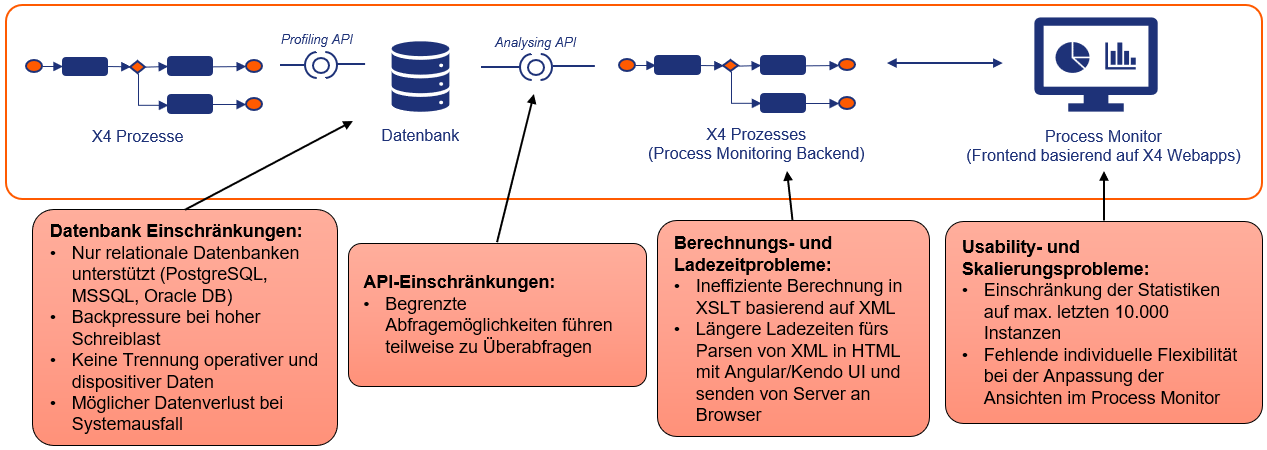
\includegraphics[width=1\linewidth]{Grafiken/Problemstellung.png}
    \caption{Darstellung der aktuellen Probleme}
    \label{fig:Problemstellung}
\end{figure}

Dabei birgt jede Phase im Datenmanagementprozess – von der Datenintegration, über Transformation und Speicherung bis hin zur Datenanalyse und Visualisierung – weitere spezifischere Herausforderungen und interdisziplinäre Fragestellungen mit sich. Diese Herausforderungen betreffen technische Aspekte wie Skalierbarkeit, Performance, Flexibilität und Integration sowie wirtschaftliche Faktoren wie Implementierungskosten, Time-to-Market, oder Kosten-Nutzen-Vergleich der Technologien.

Die Masterarbeit verfolgt das Ziel, diese komplexen Fragestellungen effizient auf ein reales Anwendungsszenario zu übertragen. Dabei wird untersucht, wie verschiedene disziplinäre Ansätze der Wirtschaftsinformatik – einschließlich Use-Case- und Systemanalyse, Technologieauswahl, Implementierung und Performanceoptimierung – kombiniert werden können, um eine effektive und skalierbare Datenmanagementlösung für die X4 BPMS zu entwickeln.

\section{Stand der Forschung}

Die vorliegende Arbeit widmet sich interdisziplinären Fragestellungen im übergeordneten Gebiet des Data Engineering, wobei der Fokus auf dem spezifischeren Kontext der Echtzeit Geschäftsprozessüberwachung mit großen Datenvolumina liegt. Es gibt bereits dedizierte Forschungsarbeiten die relevante Teilgebiete der Arbeit im Detail betrachten und Übersichtswerke die generelle Trends und Praktiken in beleuchten. Des weiteren gibt es Anbieter von Geschäftsprozessautomatisierungssoftware wie Camunda, Appian, Flowable, Mendix oder OutSystems, die im gleichen Branchenumfeld wie die SoftProject GmbH Lösungen für die Prozessüberwachung anbieten, wodurch dieser Forschungsbetrag diese in speziellen Kontext der X4 BPMS auf ihre Machbarkeit und Nutzen analysiert. 

\cite{CamundaOperate}

Beispielsweise behandeln Joe Reis und Matt Hously in einem Grundlagenwerk zum Thema Data Engineering grundsätzlich relevante Phasen, Aspekte und Fragestellungen anhand des "Data Engineering Lifecycles" von der Datengenerierung über Ingestion, Transformation, Speicherung und Bereistellung bis hin zur Analyse. \cite{reis2023} 

\section{Ansatz}

\section{Aufbau der Arbeit}
Im folgenden Kapitel \ref{StandDerForschung} werden Grundlagen
dargelegt und der Stand der Forschung diskutiert. In Kapitel
\ref{Ansatz} wird der Ansatz genauer beleuchtet. Im Kapitel
\ref{Implementierung} wird die Umsetzung des Ansatzes
beschrieben. Kapitel \ref{Validierung} praesentiert Resultate und eine
Diskussion der Ergebnisse. Im Kapitel \ref{ZusammenfassungAusblick}
wird die Arbeit zusammengefasst, ein Fazit gezogen und ein Ausblick
auf zukuenftige Arbeiten gegeben.

 
